\documentclass[border=4pt]{standalone}
\usepackage{mathptmx}
\usepackage[T1]{fontenc}
\usepackage{tikz}
\usetikzlibrary{shapes.geometric,arrows.meta,positioning,fit,calc,backgrounds}
\begin{document}

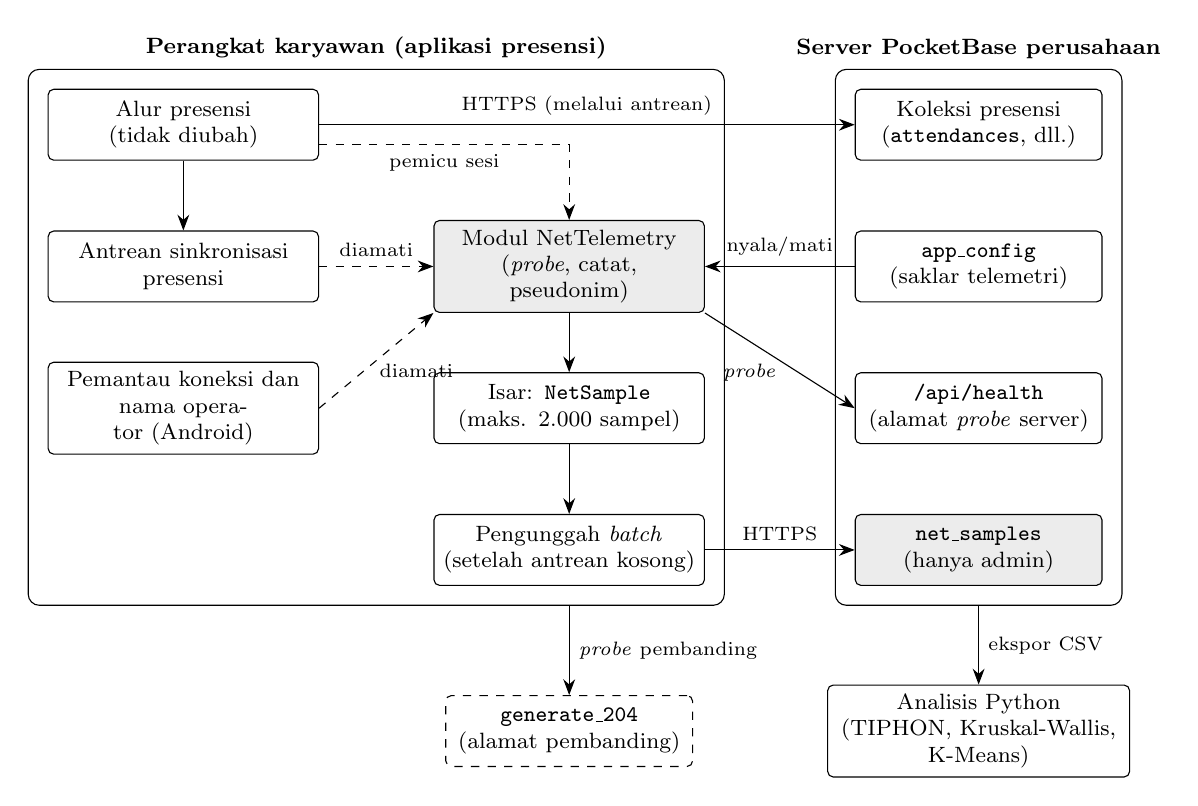
\begin{tikzpicture}[
    kotak/.style={rectangle, draw, rounded corners=2pt, align=center, text width=3.2cm, minimum height=0.9cm, font=\footnotesize},
    kotakserver/.style={rectangle, draw, rounded corners=2pt, align=center, text width=2.9cm, minimum height=0.9cm, font=\footnotesize},
    panah/.style={-{Stealth[length=2mm]}},
    amati/.style={-{Stealth[length=2mm]}, dashed}
]
% Perangkat karyawan
\node[kotak] (presensi) at (0,0) {Alur presensi\\(tidak diubah)};
\node[kotak] (antrean) at (0,-1.8) {Antrean sinkronisasi\\presensi};
\node[kotak] (koneksi) at (0,-3.6) {Pemantau koneksi dan\\nama operator (Android)};
\node[kotak, fill=gray!15] (telemetri) at (4.9,-1.8) {Modul NetTelemetry\\(\textit{probe}, catat, pseudonim)};
\node[kotak] (isar) at (4.9,-3.6) {Isar: \texttt{NetSample}\\(maks. 2.000 sampel)};
\node[kotak] (unggah) at (4.9,-5.4) {Pengunggah \textit{batch}\\(setelah antrean kosong)};
\begin{scope}[on background layer]
\node[draw, rounded corners=4pt, inner sep=7pt, fit=(presensi)(koneksi)(telemetri)(unggah), label={[font=\footnotesize\bfseries]above:Perangkat karyawan (aplikasi presensi)}] (hp) {};
\end{scope}
% Server perusahaan
\node[kotakserver] (att) at (10.1,0) {Koleksi presensi\\(\texttt{attendances}, dll.)};
\node[kotakserver] (cfg) at (10.1,-1.8) {\texttt{app\_config}\\(saklar telemetri)};
\node[kotakserver] (health) at (10.1,-3.6) {\texttt{/api/health}\\(alamat \textit{probe} server)};
\node[kotakserver, fill=gray!15] (net) at (10.1,-5.4) {\texttt{net\_samples}\\(hanya admin)};
\node[draw, rounded corners=4pt, inner sep=7pt, fit=(att)(cfg)(health)(net), label={[font=\footnotesize\bfseries]above:Server PocketBase perusahaan}] (srv) {};
% Pembanding dan analisis
\node[kotakserver, dashed] (google) at (4.9,-7.7) {\texttt{generate\_204}\\(alamat pembanding)};
\node[kotakserver, text width=3.6cm] (py) at (10.1,-7.7) {Analisis Python\\(TIPHON, Kruskal-Wallis,\\K-Means)};
% Panah
\draw[panah] (presensi) -- (antrean);
\draw[panah] (presensi) -- node[above, font=\scriptsize, pos=0.5] {HTTPS (melalui antrean)} (att);
\draw[amati] ([yshift=-0.25cm]presensi.east) -| node[below, font=\scriptsize, pos=0.25] {pemicu sesi} (telemetri.north);
\draw[amati] (antrean) -- node[above, font=\scriptsize] {diamati} (telemetri);
\draw[amati] (koneksi.east) -- node[below right, font=\scriptsize, inner sep=1pt] {diamati} (telemetri.south west);
\draw[panah] (telemetri) -- (isar);
\draw[panah] (isar) -- (unggah);
\draw[panah] (unggah) -- node[above, font=\scriptsize] {HTTPS} (net);
\draw[panah] (cfg) -- node[above, font=\scriptsize] {nyala/mati} (telemetri);
\draw[panah] (telemetri.south east) -- node[below left, font=\scriptsize, inner sep=1pt] {\textit{probe}} (health.west);
\draw[panah] (hp.south -| google) -- node[right, font=\scriptsize] {\textit{probe} pembanding} (google);
\draw[panah] (srv.south -| py) -- node[right, font=\scriptsize] {ekspor CSV} (py);
\end{tikzpicture}
\end{document}
